Ferner bietet Maven die Möglichkeit, eigene Plugins zu erstellen, womit Aufgaben und Arbeitsabläufe einfach in den Projektablauf integriert werden können, die spezifisch für das jewelige Unternehmen benötigt werden. \cite[S. 3]{varanasi_introducing_2019}

Basierend auf dem Rahmen dieser Arbeit, OSS in den DevOps-Softwareentwicklungsprozesses zu integrieren, wurde diese Möglichkeit für den PoC aufgegriffen. 

Demgemäß wurde eine entsprechende OSS als ein Maven Plugin \cite{allberg_ayoyabayoy-maven-license-verifier-plugin_2021} innerhalb des PoCs auf GitHub, einer der bekanntesten Plattformen für Quellcode-Datenbanken und deren Versionverwaltung, heruntergeladen und für den entsprechenden Verwendungszweck angepasst.

\subsubsection{Workflow Maven}

Um ein besseres Verständnis zu ermöglichen, wird zunächst auf die generelle Funktionsweise von Maven näher eingegangen. 

\begin{figure}[h]
    \centering
    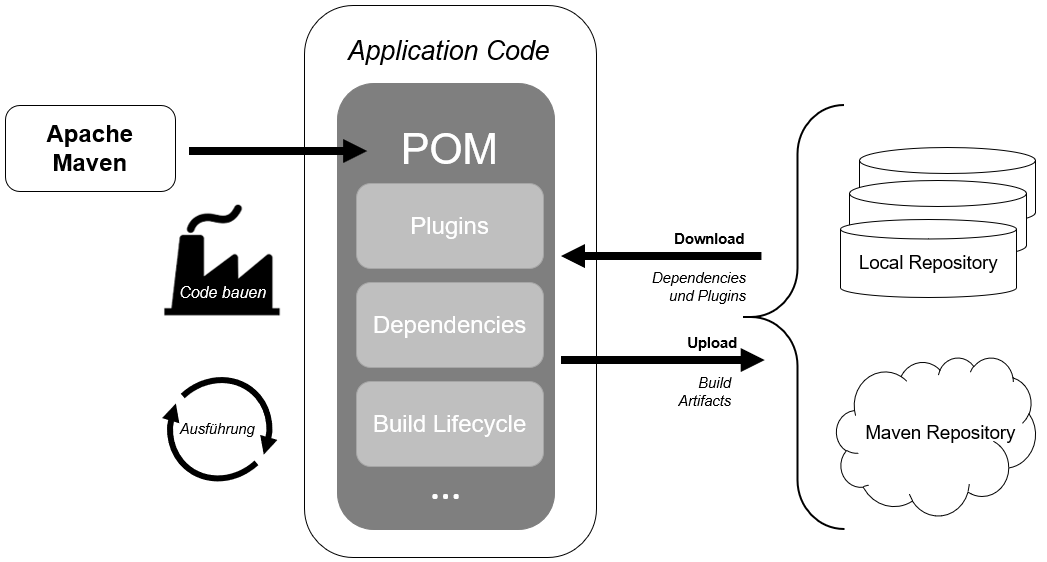
\includegraphics[scale=0.6]{Bilder/Workflow_Maven.png}
    \caption{Funktionsweise von Maven, angelehnt an \cite{guntur_understanding_2020}}
\end{figure}

\paragraph{POM}
Die Funktionsweise von Maven als auch die Verwaltung des Projektes baut grundsätzlich auf dem 'Project Object Model' (kurz: POM) auf und bildet daher den Kern eines jeden Maven-Projektes ab.

Die POM wird innerhalb der Datei pom.xml gespeichert, die wiederrum im Projektverzeichnis liegt.

Die POM beinhaltet alle notwendigen Projektinformationen, vorhandenen Abhängigkeiten, dem Quelldateiverzeichnis Konfigurationen und Plugininformationen, die während des Build-Prozesses verwendet werden sollen.\cite{the_apache_software_foundation_maven_2002}

Die POM muss drei wesentliche Tags enthalten \cite[S. 77 - 78]{spiller_maven_2011}: 

\begin{itemize}
    \item \textit{groupId}: Enthält eine eindeutige, identifizierbare Bezeichnung für ein Projekt
    \item \textit{artifactId}: Enthält eine eindeutige, identifizierbare Bezeichnung für ein Artefakt bzw. Projekt pro groupId
    \item \textit{version}: Enthält die aktuelle Version des Artefakts
\end{itemize}

Alle weiteren definierten Eigenschaften werden von der Super-POM vererbt, welches die Standardkonfigurationen, Plugins und Verzeichnisse enthält.

Entscheidend ist, dass Maven keine vollständigen Projekte, sondern eigenständige Projektteile, also Artefakte beschreibt, die einzeln ausgeliefert werden. \cite[S. 29]{spiller_maven_2011}

Demzufolge erzeugt jedes Maven-Projekt ein Artefakt, welches auf die Repositorys übertragen wird. 

\paragraph{Repository}

Ferner verwendet Maven das 'Local Repository' und das konfigurierte 'Maven Repository'.

Innerhalb des Local Repositorys werden alle Abhängigkeiten abgelegt, die für die Erstellung des Builds benötigt werden. 

Zunächst überprüft Maven bei der Zerlegung der Abhängigkeiten, ob sich die benötigten Dateien bereits innerhalb des Local Repositorys befinden. \cite[S. 45 - 47]{loukides_maven_2008} 

Ist dies der Fall, wird die Datei, ohne die Erstellung einer Kopie im lokalen Verzeichnis, innerhalb des Local Repositorys verwendet.

Kann keine Zerlegung der Abhängigkeiten lokal erfolgen, versucht Maven diese mittels dem Maven Repository über das Internet auf das Local Repository herunterzuladen und zu kopieren, damit diese aussschließlich lokal verwendet werden.\cite[S. 115]{spiller_maven_2011}   

Sollten neue Abhängigkeiten oder neue Versionen der vorhandenen Abhängigkeiten hinzugefügt werden, wird das Repository anhand dessen aktualisiert oder die betreffenden Abhängigkeiten kopiert. 

Die Abhängigkeiten, also die genutzten Bibliotheken werden in der pom.xml definiert. 

\paragraph{Build-Lifecycle}

Prinzipiell sind Lifecycles abstrahierte Arbeitsschritte innerhalb festen Phasen, die in einer bestimmten Reihenfolge durchlaufen und für den Build-Prozess essentiell sind. \cite[S. 57]{varanasi_introducing_2019}  

Durch das standardisierte Vorgehen, lässt sich das Ararbeiten der Aufgaben verallgemeinern und vereinheitlichen, was für den Entwickler unterstützend ist.

Maven definiert dabei drei Lifecycles\cite[S. 72 - 76]{spiller_maven_2011}: 

\begin{itemize}
    \item \textit{clean}\\
    Mittels dieses Lifecycles wird alles gelöscht, was keine Notwendigkeit mehr hat, so wie beispielsweise die vom vorherigen Build erstellten Dateien. 

    \item \textit{site}\\
    Innerhalb dieses Lifecycles umfasst alle Phasen, die zum Erzeugen einer Projektdokumentation benötigt werden.
    
    \item \textit{build/default}\\
    Dieser Lifecycle stellt den standardisierten Ablauf aller Phasen dar, die nach dem Aufruf von Maven zum Übersetzen und Erzeugen einer Anwendung abgearbeitet werden. 
    
    Dieser enthält acht wesentliche Phasen, die nach einer unveränderbaren Reihenfolge abgearbeitet werden: validate, compile, test, package, integration-test, verify, install und deploy.  

\end{itemize}

Folglich muss bei einem Aufruf einer bestimmten Phase, die vorangegangen Phasen ebenfalls abgearbeitet werden. 

Neben den Phasen sind auch die zugrundeliegenden Plugins innerhalb jedes Lifecycles verbunden, die sich wiederrum durch das Ausführen von Plugin-Goals in den einzelnen Phasen modefizieren lassen. \cite[S. 71]{spiller_maven_2011}

\begin{figure}[h]
    \centering
    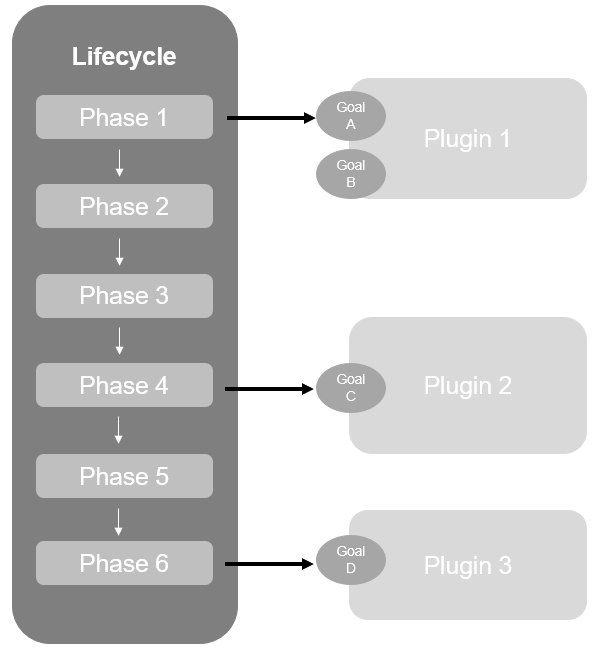
\includegraphics[scale=0.6]{Bilder/lifecycle_maven.png}
    \caption{Zusammenspiel Plugin-Goals und Lifecycle, \cite[S. 59]{varanasi_introducing_2019}}
\end{figure}

Sobald Maven die einzelnen Phasen eines Lifecycles durchläuft, werden die Ziele ausgeführt, die mit jeder einzelnen Phase verbunden sind. \cite[S. 39]{loukides_maven_2008} 

Infolgedessen werden bestimmte Funktionalität eines Plugins durch das entsprechende Goal bestimmt. 

Während das POM alle notwendigen Informationen über ein Projekt enthält, die während des Build-Prozesses verwendet werden sollen, also das "Wer", "Was" und "Wo", stellt der Lifecycle das "Wann" und "Wie" dar. \cite{the_apache_software_foundation_maven_2002}

\paragraph{Plugins in Maven}





% Maven  wurde  so  konzipiert,  dass  die meisten  Funktionen  von  Plugins  geliefert  werden.  Die  Grundfunktionen  beinhalten  etwa  das Parsen  von XML-Dateien,  Plugin-Verwaltung  und  den Default-Lifecycle.  

% Das  heißt  dass  die Hauptverantwortung  auf  Plugins  fällt. 

% Auch  andere  wichtige  Funktionen  wie  das  Kompilieren  des  Projektes  sind nicht Bestandteil derGrundfunktionenvon Maven. 

% Jede Phase kann von einem Plugin „ersetzt“ werden. 

% Maven  hat  also  verschiedene  Aufgaben  als  Plugins  ausgelagert.

% Dies  hatden  Vorteil,dass einzelne Plugins mit bestimmten Aufgaben weitaus leichterzu Warten und Einzusetzen sind, als große Bibliotheken.

% Der Nutzer muss nichts tun um Updatesder Pluginszu erhalten, da dies von Maven  geregelt  wird.Das  heißt  gleichzeitig  auch  dass  der  Nutzer  in  seinem  Projekt so  gut  wie keine   Anpassungen   am   Projektcode   machen   muss   um   neuen   Code   zu   unterstützen, vorrausgesetzt   die   Abwärtskompatibilität des Plugins   ist   erhalten   geblieben.   

% Die   einzige Benötigte Anpassung ist die Versionsnummer des jeweiligen Plugins in der Projekt-POM.Wird in der   POM   eine   neue   Version   eingetragen,   wird   diese   automatisch   ins   lokale   Repository heruntergeladen und benutzt

\paragraph{Abhängigkeiten verwalten mittels Dependencies-Dateien}

\subsubsection{Entwurf PoC basierend auf einem Maven-Plugin}
%Idee: Lizenzen als eine Datei zu beschreiben und mit den Lizenzen die sich in den Dependency-Dateien befinden, zu vergleichen 



